In this chapter the planning and work-flow regarding Sprint 3 will be described. 
Everything from setting our goals to implementation and testing. At the end we will evaluate the whole sprint, and try to answer on following questions: What went well? What could be improved? What should we start doing?  
% TODO rewrite

\section{Sprint planning}
In the planning part of sprint 2, there have been introduced and idea or goal for refining and extending the existing code, customer agreed, with condition, that sprint 3 will be focused on image processing part.

As the image processing module was one of the major risks, there was done some preliminary research even in the end of sprint 2 about possible approaches.
One specific way to deal with the problem (using OpenCV and Hough transformation \cite{Duda:1972:UHT:361237.361242}) was introduced to customer in planning part of meeting.
Customer was not satisfied with such a low-level approach and wanted us to use some existing tools.
Therefore there was need for additional preliminary studies concerning existing projects or libraries that could be used.
You can read more about additional preliminary studies below.

Also there was made a proposal of additional "pre-demo" video showing the progress of implementation on Thursday 4th of October 2013 during the regular meeting and customer gladly accepted this offer.


\subsection{Duration}
This sprint is 2 weeks long. From 30th of September 2013 to 13th of October 2013.
We agreed on the date of presentation and showing the running demo -- on Thursday 11 of October 2013.
Estimated velocity is 240 hours since we agreed on 30 working hours per person per week.

\subsection{User-stories}

\subsubsection*{Implementation}
All the functional requirements for sprint 3 are presented in Table \ref{tab:sprint3stories}
\LTXtable{\textwidth}{sprint3/stories.tex}

\subsubsection*{Documentation}
All the documentation stories for sprint 3 are presented in Table \ref{tab:sprint3Documentationstories}
\LTXtable{\textwidth}{sprint3/storiesDocumentation.tex}

\subsubsection*{Project management}
All the project management for sprint 3 are presented in Table \ref{tab:sprint3storiesProcess}
\LTXtable{\textwidth}{sprint3/storiesProcess.tex}
% hous all in total: Estimated: 94+ 94 + 50= 238 Spent: 97+ 86+ 36 = 219
\section{Preliminary studies}
% TODO

\section{Sprint goal}
The goal of this sprint is having a working application on a mobile phone that can work in two modes.  
Input type and output are for both modes common -- input is an image or video and output is location of detected mobile phones in a given matrix (e.g. 4x4 matrix) with color that mobile's screen is lighting.
In the first mode, real video from mobile's camera will be treated as an input and on the other hand in the second mode mock data (image or video) are treated as an input.

You can see example of input with matrix 2x2 in Figure \ref{img:sprint3_goal}. Appropriate output of image processing and mapping module is: \texttt{\{blue,[0,0]\}, \{red,[1,0]\}, \{green,[0,1]\}}.

\begin{figure}[H]
	\centering
		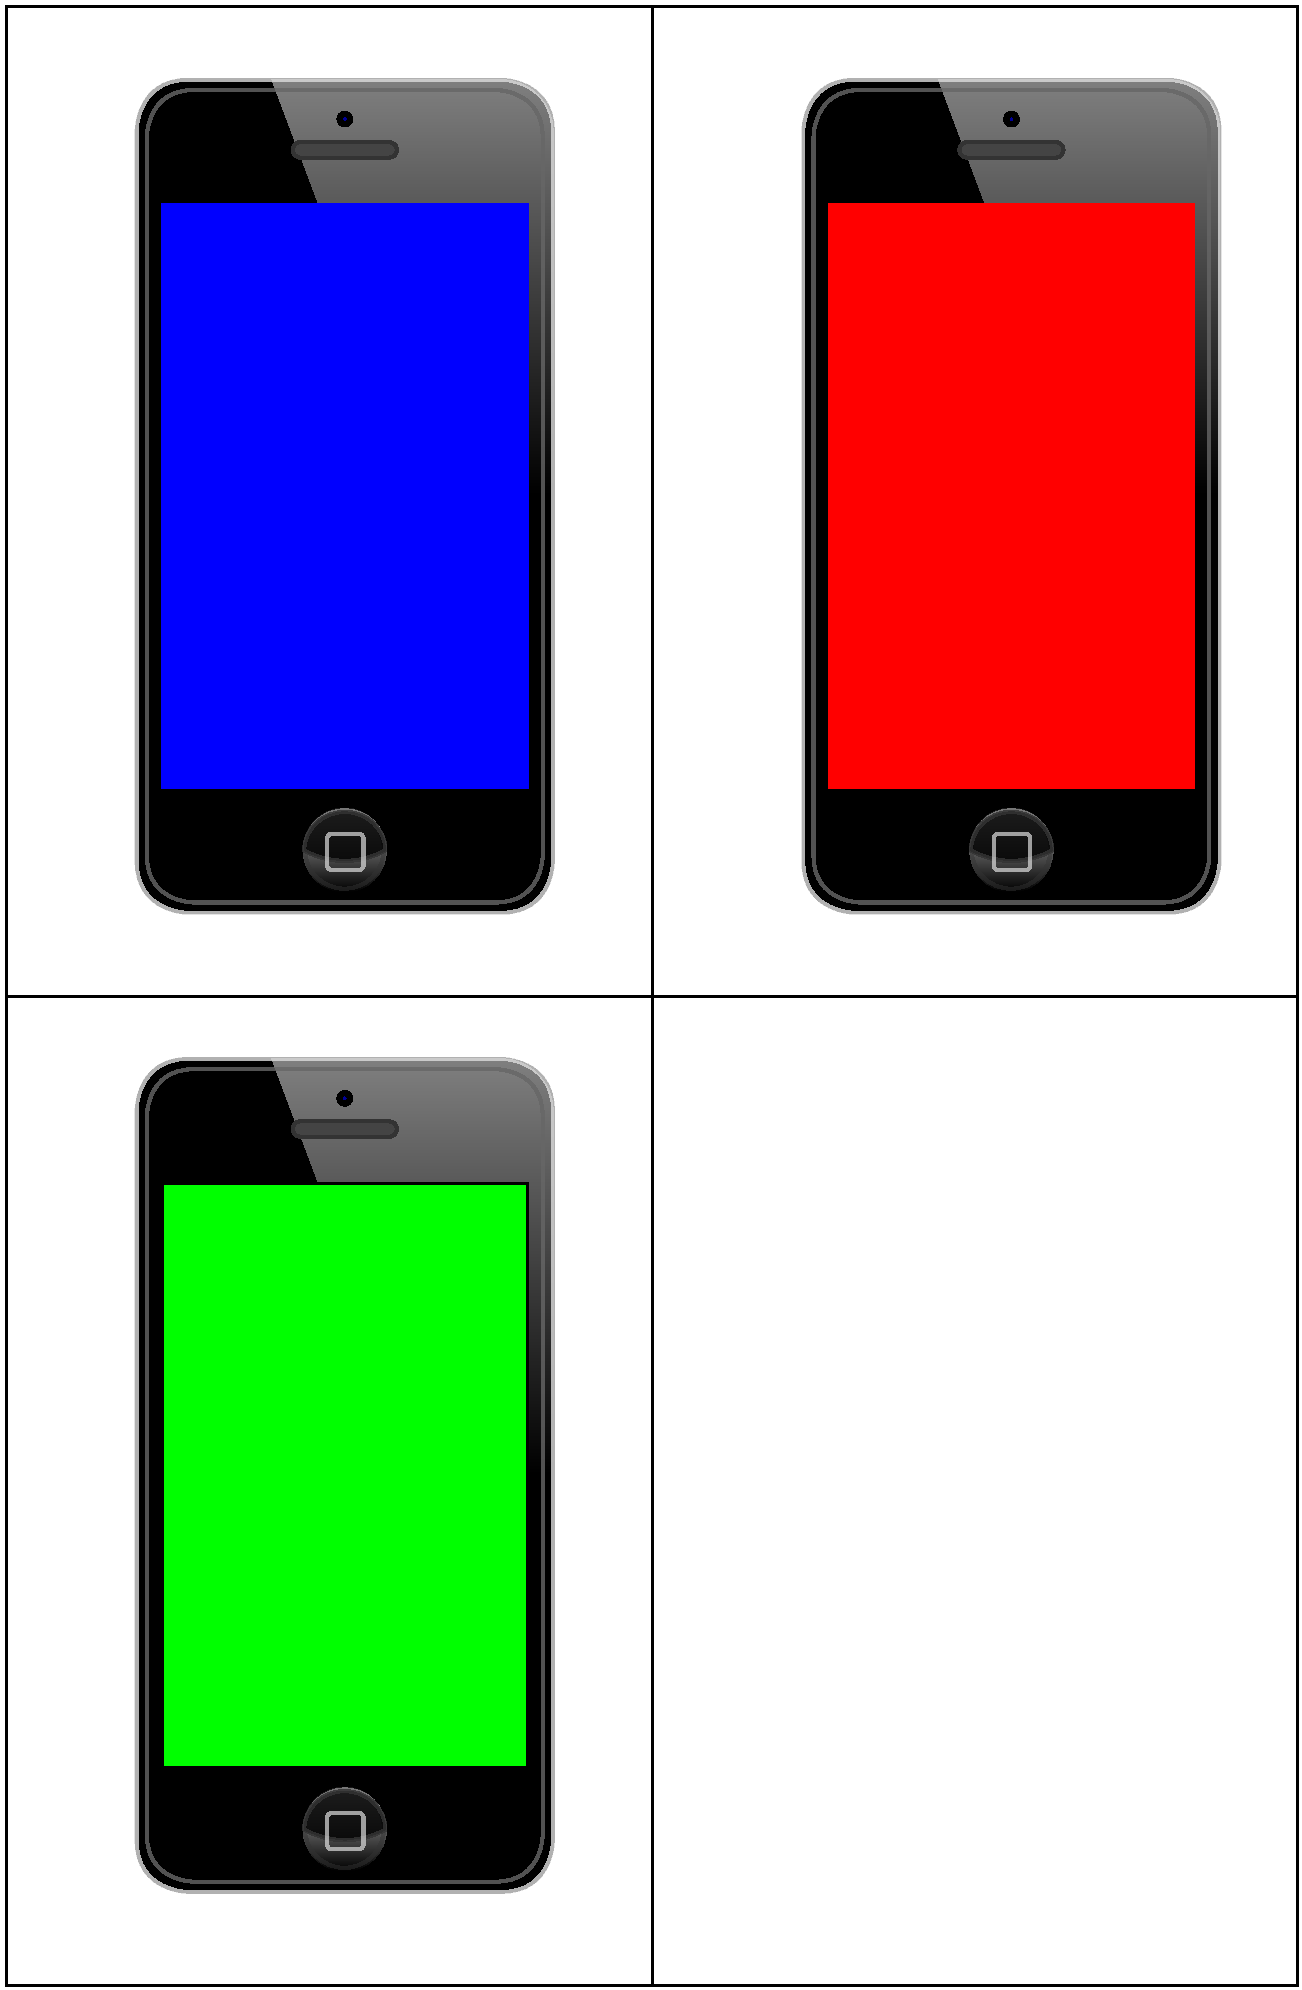
\includegraphics[width=7cm]{sprint3/sprint3_goal.pdf}
	\caption{Example of ideal data input for image processing module with 2x2 matrix}
	\label{img:sprint3_goal}
\end{figure}

\section{System Burndown}
\begin{figure}[H]
	\centering
		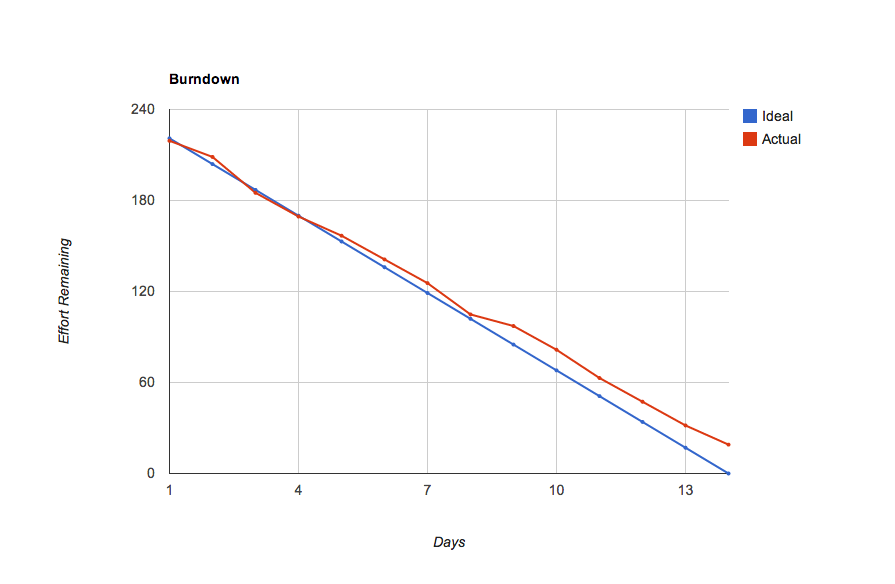
\includegraphics[width=18cm]{sprint3/BurndownSprint3.png}
	\caption{Burn down chart}
	\label{fig:Burn3 }
\end{figure}

\section{Architecture}
In this section will be described image processing module using 4+1 architectural view module.

\subsection{Logical view}
You can see a class diagram of new classes created in sprint 3 in Figure \ref{fig:class_diagram_sprint3}. We can divide these new classes into three categories. 

Into the first category we count classes \texttt{LightDetector}, \texttt{TileMapper} and \texttt{PointCollector}. 
These classes are a core of image processing module. 
The only visible method for working with this module is \texttt{PointCollector}'s method \texttt{collect}.
This function accepts two parameters: first is the image where mobile phone's screen detection should be done and second is a list of colors of screens which should be detected. 
Method \texttt{collect} is run asynchronously (as a new thread due to possible high time demanding operations) and therefore it was designed as a design pattern \texttt{Observer}
As class \texttt{PointCollector} implements interface \texttt{Observable} (also known as a \emph{Subject} \cite[p.~326]{Gamma:1995:DPE:186897}), its \texttt{Observers} must implement method \texttt{update}. 
To this function is passed as a argument hash map with keys as a colors and values as a lists of tile positions with appropriate color.
Class \texttt{LightDetector} is responsible for detecting location of color blobs in given image. 
Results as a list of pixel's position of blobs are passed as a return value of function \texttt{getBlobCoords}. 
These values are fetched by instance of \texttt{PointCollector} and passed to \texttt{TileMapper}, which is responsible for mapping points into appropriate tiles in grid.

In second category there is only class \texttt{CameraActivity}, who is responsible for handling outputs from camera or mock device and also gives appropriate feedback on screen of mobile (draws grid and marks detected blobs).

In last category there is class \texttt{ColorManager}, which is standalone class and in application there is only need for one instance. Therefore it was designed as a \texttt{Singleton} pattern \cite[p.~144]{Gamma:1995:DPE:186897}. Its main purpose is to handle transformations of different color formats such as special library, network and internal formats.

\begin{figure}[H]
	\centering
		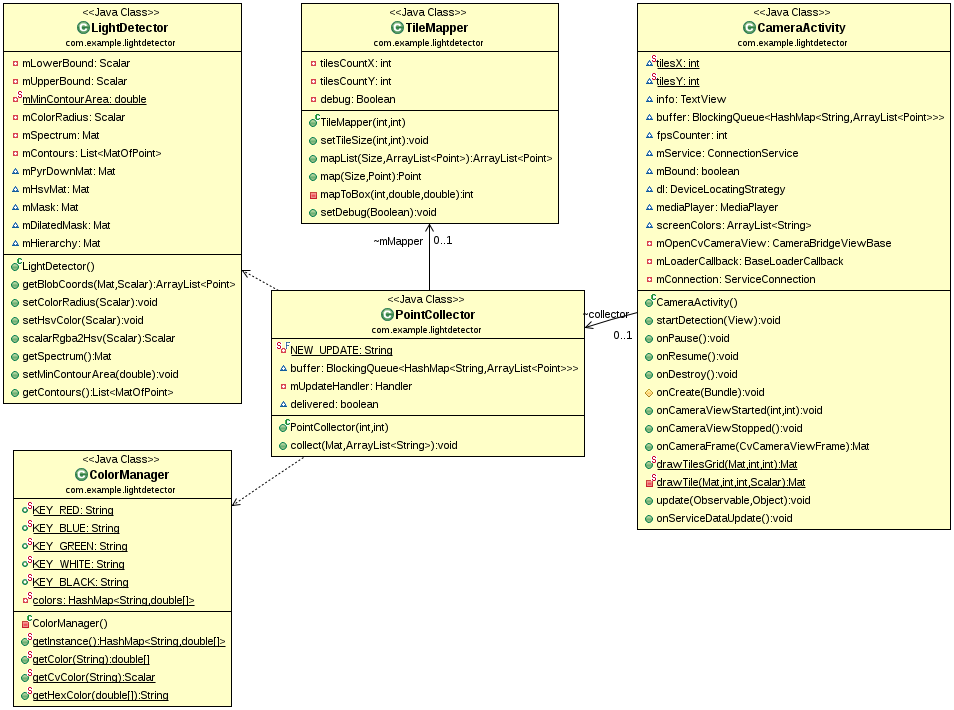
\includegraphics[width=16.2cm]{sprint3/sprint3.png}
	\caption{Sprint 3 light detection module class diagram}
	\label{fig:class_diagram_sprint3}
\end{figure}

\subsection{Physical view}
You can see the physical view of whole product represented in Figure \ref{fig:sprint3_deployment_diagram}.
Even though in this particular case device \emph{Camera} part of \emph{Server} device, the architecture and code was designed generally so \emph{Camera} can be stand alone device.

\begin{figure}[H]
	\centering
		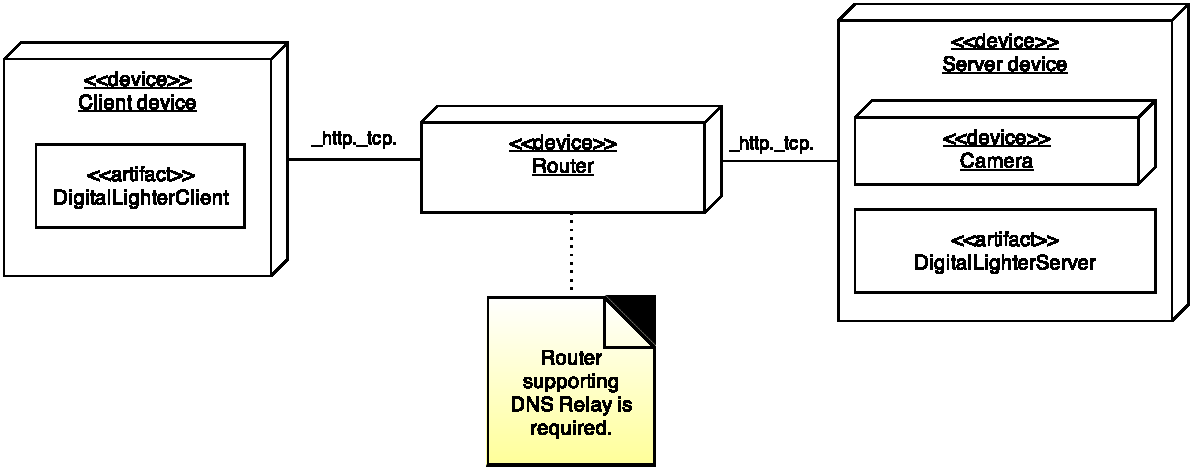
\includegraphics[width=15cm]{images/deployment-diagram-sprint3}
	\caption{Deployment diagram}
	\label{fig:sprint3_deployment_diagram}
\end{figure}

\subsection{Process view}
You can see the process view represented in Figures \ref{fig:sprint3_activity_diagram} and \ref{fig:sprint3_dfd}.
It should be mentioned, that each time new image was taken by camera, new thread is created and therefore several processing in the same time can be performed.

\begin{figure}[H]
	\centering
		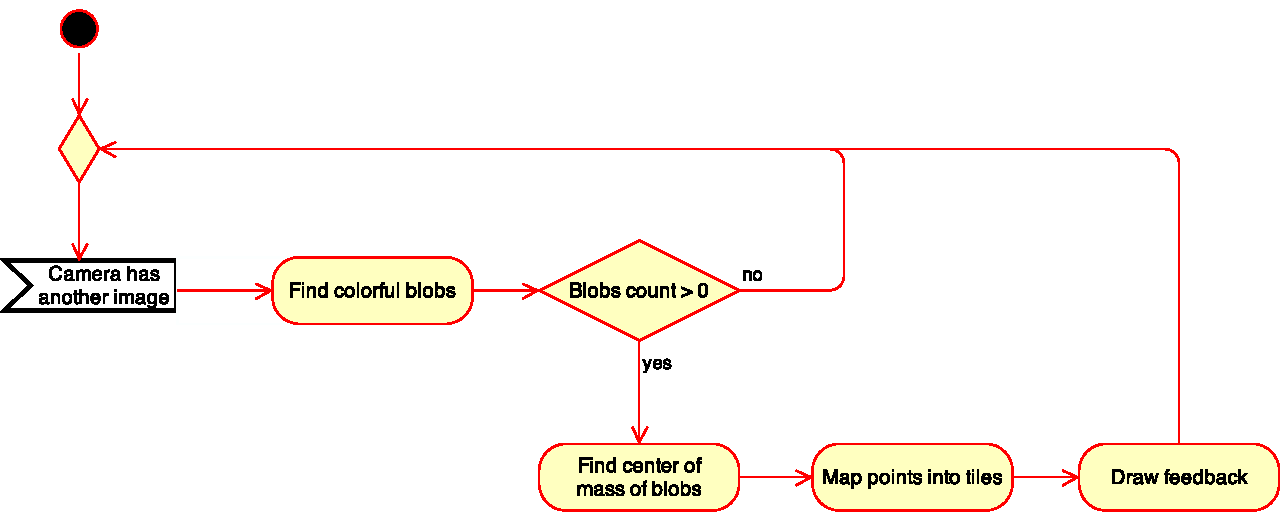
\includegraphics[width=16.2cm]{sprint3/activity_sprint3.pdf}
	\caption{Sprint 3 activity diagram}
	\label{fig:sprint3_activity_diagram}
\end{figure}


\begin{figure}[H]
	\centering
		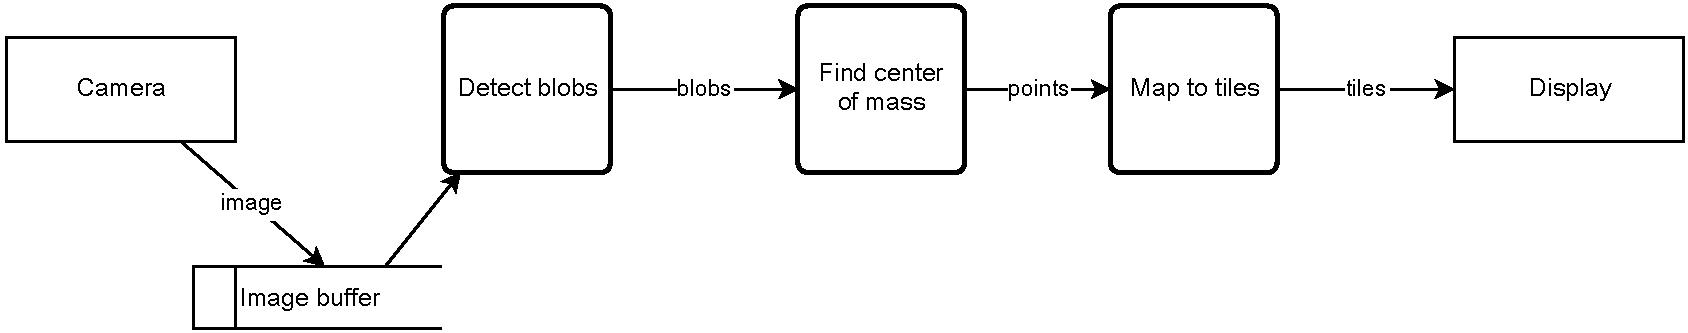
\includegraphics[width=16.2cm]{sprint3/sprint3_dtd.pdf}
	\caption{Sprint 3 data flow diagram}
	\label{fig:sprint3_dfd}
\end{figure}

%\subsection{Development view}
%Since this is a single module, there is no need for development view

\section{Implementation}

Few problems during implementation had occurred. 
Since the OpenCV library for Java is in early stage, there is some functionality missing.
One of these is a method \texttt{open(String)} of class \texttt{VideoCapture}\footnote{http://docs.opencv.org/java/org/opencv/highgui/VideoCapture.html}.
In C++ version of OpenCV there exist such a method and it allows programmers to use a video for input for image processing.
After short research, a fix of this bug was found\footnote{http://code.opencv.org/issues/3207}, but this feature will be added in release 2.4.7.
Due to this discovery, there has been abandoned (at least until OpenCV 2.4.7 is released) a plan for mocking a video and only single pictures were used for testing.


\section{Testing}
A capability of Java to run on multiple platforms were utilized during testing and initial testing was performed without any Android device.
There have been created a testing set\footnote{https://github.com/dohnto/DigitalLighter/tree/master/source/others/LightDetectorTester/res/drawable} of simple images used for black box testing.

After this test, it has been decided to merge module with the rest of the application and perform some integration tests.
To outline a characteristics of further testing you can see videos \footnote{http://www.youtube.com/watch?v=TcuMlvvAwSQ} \footnote{http://www.youtube.com/watch?v=fhWFAJY7QOg} demonstrating current progress of implementation.

\section{Occurring risks}
This sprint, the \emph{dead end with technology} risk occurred. 
Since the required functionality (loading mocked videos) was proposed by customer mainly from testing reasons, the fact that the team met dead end was announced to customer with proposition, that the team can spend more time on researching other solutions or simply the final product will lack this feature.
The customer have chosen second choice.

\section{Customer feedback}
Since the pre-demo video was presented to customer during regular meetings, 

\section{Retrospective}
This section reflects on the past sprint. In order to learn from the mistakes done and thus to improve the workflow it is necessary to answer two essential questions: "What went well" and "What could be improved".

\subsection{What went well}
Since the preliminary studies concerning image processing started very soon and instead of writing light detection module from scratch an existing code was used, the core of implementation was finished ahead of schedule.

\subsection{What could be improved}
Due to misunderstanding about customer's demands regarding using existing solution, extra time was required for additional preliminary studies resulting to the same output as the first preliminary study concerning image processing. 

In the end, the customer approved using OpenCV as a best option.
Therefore the communication with customer should be more precise and accurate and if any ambiguity occurs, it should be consulted with customer as soon as possible.

From the beginning it was obvious, that the light detection module's performance affected by level of light.
During the testing the team was uncertain when the performance is sufficient, because the question of lighting was not discussed enough.
After this experience, an proposal to customer was made: if similar situation occurs, acceptance tests should be prepared and approved by the customer.

Last but not least, documentation stories XX YY ZZ were not finished due to need to refining previously written chapters.

Also, daily stand ups were often omitted due to late attendance.
Even though the workload is 30 hours per week per person, the efficiently spend time is much lower, therefore the workload was decreased to 25 hours per week per person (it better reflects the reality).
